\documentclass[11pt]{article} 
\usepackage[english]{babel}
\usepackage[utf8]{inputenc}
\usepackage[margin=0.5in]{geometry}
\usepackage{amsmath}
\usepackage{amsthm}
\usepackage{amsfonts}
\usepackage{amssymb}
\usepackage[usenames,dvipsnames]{xcolor}
\usepackage{graphicx}
\usepackage[siunitx]{circuitikz}
\usepackage{tikz}
\usepackage{tkz-berge}
\usetikzlibrary{positioning, automata, backgrounds}
\usepackage{tikz-qtree}
\usepackage[colorinlistoftodos, color=orange!50]{todonotes}
\usepackage{hyperref}
\usepackage[numbers, square]{natbib}
\usepackage{fancybox}
\usepackage{epsfig}
\usepackage{soul}
\usepackage[framemethod=tikz]{mdframed}
\usepackage[shortlabels]{enumitem}
\usepackage[version=4]{mhchem}
\usepackage{multicol}
\usepackage{forest}
\usepackage{mathtools}
\usepackage{comment}
\usepackage{enumitem}
\usepackage[utf8]{inputenc}
\usepackage{listings}
\usepackage{color}
\usepackage[numbers]{natbib}
\usepackage{subfiles}
\usepackage{tkz-berge}
\usepackage{algorithm}
\usepackage[noend]{algpseudocode}


\newtheorem{prop}{Proposition}[section]
\newtheorem{thm}{Theorem}[section]
\newtheorem{lemma}{Lemma}[section]
\newtheorem{cor}{Corollary}[prop]

\theoremstyle{definition}
\newtheorem{definition}{Definition}

\theoremstyle{definition}
\newtheorem{required}{Problem}

\theoremstyle{definition}
\newtheorem{ex}{Example}

\newcommand{\interval}[4]{\draw (#2, #1) -- (#3, #1); % Usage: \interval{height}{start}{end}{label}
\draw (#2, #1-0.11) -- (#2, #1+0.11); % draw left whisker
\draw (#3, #1-0.11) -- (#3, #1+0.11); % draw right whisker
\node[] at (#2-0.25, #1) {#4};
}


\setlength{\marginparwidth}{3.4cm}
%#########################################################

%To use symbols for footnotes
\renewcommand*{\thefootnote}{\fnsymbol{footnote}}
%To change footnotes back to numbers uncomment the following line
%\renewcommand*{\thefootnote}{\arabic{footnote}}

% Enable this command to adjust line spacing for inline math equations.
% \everymath{\displaystyle}

% _______ _____ _______ _      ______ 
%|__   __|_   _|__   __| |    |  ____|
%   | |    | |    | |  | |    | |__   
%   | |    | |    | |  | |    |  __|  
%   | |   _| |_   | |  | |____| |____ 
%   |_|  |_____|  |_|  |______|______|
%%%%%%%%%%%%%%%%%%%%%%%%%%%%%%%%%%%%%%%

\title{
\normalfont \normalsize 
\textsc{CSCI 3104 Fall 2021 \\ 
Instructors: Profs. Grochow and Waggoner} \\
[10pt] 
\rule{\linewidth}{0.5pt} \\[6pt] 
\huge Problem Set 11 \\
\rule{\linewidth}{2pt}  \\[10pt]
}
%\author{Your Name}
\date{}

\begin{document}
\definecolor {processblue}{cmyk}{0.96,0,0,0}
\maketitle


%%%%%%%%%%%%%%%%%%%%%%%%%
%%%%%%%%%%%%%%%%%%%%%%%%%%
%%%%%%%%%%FILL IN YOUR NAME%%%%%%%
%%%%%%%%%%AND STUDENT ID%%%%%%%%
%%%%%%%%%%%%%%%%%%%%%%%%%%
\noindent
Due Date \dotfill TODO \\
Name \dotfill \textbf{Your Name} \\
Student ID \dotfill \textbf{Your Student ID} \\
Collaborators \dotfill \textbf{List Your Collaborators Here}

\tableofcontents

\section{Instructions}
 \begin{itemize}
	\item The solutions \textbf{must be typed}, using proper mathematical notation. We cannot accept hand-written solutions. \href{http://ece.uprm.edu/~caceros/latex/introduction.pdf}{Here's a short intro to \LaTeX.}
	\item You should submit your work through the \textbf{class Canvas page} only. Please submit one PDF file, compiled using this \LaTeX \ template.
	\item You may not need a full page for your solutions; pagebreaks are there to help Gradescope automatically find where each problem is. Even if you do not attempt every problem, please submit this document with no fewer pages than the blank template (or Gradescope has issues with it).

	\item You are welcome and encouraged to collaborate with your classmates, as well as consult outside resources. You must \textbf{cite your sources in this document.} \textbf{Copying from any source is an Honor Code violation. Furthermore, all submissions must be in your own words and reflect your understanding of the material.} If there is any confusion about this policy, it is your responsibility to clarify before the due date. 

	\item Posting to \textbf{any} service including, but not limited to Chegg, Reddit, StackExchange, etc., for help on an assignment is a violation of the Honor Code.

	\item You \textbf{must} virtually sign the Honor Code (see Section \ref{HonorCode}). Failure to do so will result in your assignment not being graded.
\end{itemize}


\section{Honor Code (Make Sure to Virtually Sign)} \label{HonorCode}

\begin{required}
\begin{itemize}
\item My submission is in my own words and reflects my understanding of the material.
\item Any collaborations and external sources have been clearly cited in this document.
\item I have not posted to external services including, but not limited to Chegg, Reddit, StackExchange, etc.
\item I have neither copied nor provided others solutions they can copy.
\end{itemize}

%\noindent In the specified region below, clearly indicate that you have upheld the Honor Code. Then type your name. 
\end{required}

\begin{proof}[Agreed (signature here).]
%% Typing "I agree to the above," followed by your name is sufficient.
\end{proof}


\newpage
\section{Standard 24- Dynamic Programming: Design DP Algorithms}

\begin{required}
The \textsf{Placing Electrons on a Tree} problem is defined as follows. 
\begin{itemize}
\item \textsf{Instance:} A tree rooted tree $T$, with root $r \in V(T)$.
\item \textsf{Solution:} A subset $S \subseteq V(T)$ such that there are no edges $(s,s')$ for $s,s' \in S$, and such that $|S|$ is as large as possible.
\end{itemize}
The \emph{idea} is that you are placing electrons on the vertices of a tree, but electrons repel each other, so you cannot place two electrons adjacent to one another, with the goal being to place as many electrons as possible.

\noindent \\ The goal of this problem set is to design a dynamic programming algorithm to solve the \textsf{Placing Electrons on a Tree} problem.

\begin{enumerate}[label=(\alph*)]
\subsection{Problem 2\ref{2a}}
\item \label{2a} For each vertex $v \in V(T)$, let $L[v]$ denote the maximum number of electrons that can be placed on the subtree rooted at $v$. Write down a mathematical recurrence for $L[v]$. Clearly justify each case. \emph{Hint:} your recurrence should involve the children and grandchildren of $v$. You may use notation such as ``children$(v)$'' to denote the set of children of $v$, and ``grandchildren$(v)$'' to denote the set of grandchildren of $v$. Remember to have base case(s).

\begin{proof}[Answer]
%Your answer here
\end{proof}



\newpage
\subsection{Problem 2\ref{2b}}
\item \label{2b} Clearly describe how to construct and fill in the lookup table. For the cell $L[v]$, clearly describe the sub-cases we consider, and which optimal sub-case we select. \emph{Hint:} Similar to counting paths in a DAG, what order should you put the vertices in so that you can fill in the lookup table ``in order''?

\begin{proof}[Answer]
%Your answer here
\end{proof}

\newpage
\subsection{Problem 2\ref{2c}}
\item \label{2c} Let \texttt{back}$[v]$ denote another array storing ``backpointer'' information to enable you to reconstruct the optimal solution. Clearly describe what information should be stored in \texttt{back}[v] and how it is generated based on the optimal sub-cases selected in the computation of $L[v]$ (as you described in Problem2\ref{2b} above).


\begin{proof}[Answer]
%Your answer here
\end{proof}

\newpage
\subsection{Problem 2\ref{2d}}
\item \label{2d} Work through an example of your algorithm using the following tree. Clearly show how to recover an optimal solution using your lookup table. You may hand-draw your lookup table, but your explanation must be typed.

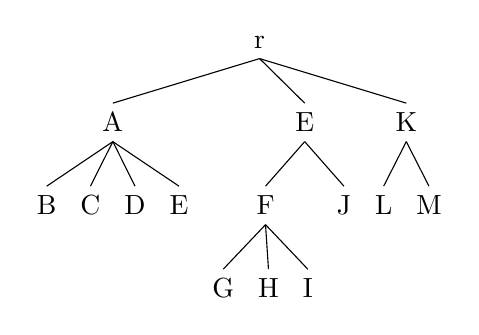
\begin{tikzpicture}
\Tree [.r [. A B C D E ] 
             [. E [. F G H I ] J ]
             [. K L M ] ]
\end{tikzpicture}


\begin{proof}[Answer]
%Your answer here
\end{proof}

\end{enumerate}



\end{required}

\end{document} % NOTHING AFTER THIS LINE IS PART OF THE DOCUMENT



